\documentclass[12pt]{ctexart}
\usepackage{config}

%LaTeX模板作者：GitHub@nsyhfxc
%请勿修改config.sty的设置,否则会导致格式混乱


\newcommand{\SoftwareName}{文本背诵记忆助手软件} %填软件名称
\newcommand{\DocType}{设计说明} %这里区分是设计说明还是使用说明
\newcommand{\Version}{V1.0} %版本号是V1.0
\newcommand{\Authors}{钟睿洁} %作者姓名
\newcommand{\CreatDate}{2026年3月21日} %文档创建时间
\newcommand{\UpdateDate}{\today} %文档更新时间

%这里是全局文本设置,相关文本仅需设置一次即可


\begin{document}


\maketitle

\vspace{10cm}

%此表自动生成，无需改动

\begin{table}[H]
\centering
\begin{tabular}{|m{0.28\textwidth}|m{0.68\textwidth}|}
	\hline
	版本: & \Version \\
	\hline
	文档状态： & 编辑 \\
	\hline
	作者： & \Authors \\
	\hline
	负责人： & \Authors \\
	\hline
	创建日期： & \CreatDate \\
	\hline
	更新日期： & \UpdateDate \\
	\hline
\end{tabular}
\end{table}

\newpage

\begin{center}
	\zihao{3}
	\textbf{修订记录}
	\vspace{-1em}
\end{center}

\begin{table}[H]
\centering
\renewcommand{\arraystretch}{1.25}
\setlength{\tabcolsep}{0pt}
\setlength{\dashlinedash}{1pt}
\setlength{\dashlinegap}{2pt}
\begin{tabular}{
	|>{\centering\arraybackslash}p{0.25\textwidth}:
	>{\centering\arraybackslash}p{0.2\textwidth}:		>{\centering\arraybackslash}p{0.25\textwidth}:
	>{\centering\arraybackslash}p{0.3\textwidth}|
	}
	\hline
	\textbf{日期} & \textbf{版本} & \textbf{修改者} & \textbf{描述} \\
	\hdashline
	2025--12--11 & 0.7 & \Authors & XXXX \\
	\hdashline
	2025--12--14 & 0.8 & \Authors & XXXX \\
	\hdashline
	2025--12--20 & 0.9 & \Authors & XXXX \\
	\hdashline
	2026--02--27 & 1.0 & \Authors & XXXX \\
	\hdashline
	&  &  &  \\
	\hdashline
	&  &  &  \\
	\hdashline
	&  &  &  \\
	\hdashline
	&  &  &  \\
	\hdashline
	&  &  &  \\
	\hdashline
	&  &  &  \\
	\hline
\end{tabular}
\end{table}


\newpage

\tableofcontents

\newpage %包括封面设置、修订记录、目录

\section{申请流程(此部分仅供流程介绍,不在最终提交材料中)}

\subsection{注册申请账号}

点击下面的链接即可进入版权保护中心的用户中心登录页面：

\url{https://register.ccopyright.com.cn/account.html?current=soft_register}

注册完成后需要进行实名认证，需要大约3个工作日审核。审核完成后，即可开始登记软件著作权。


\subsection{软著登记}


\begin{figure}[H]
	\centering
	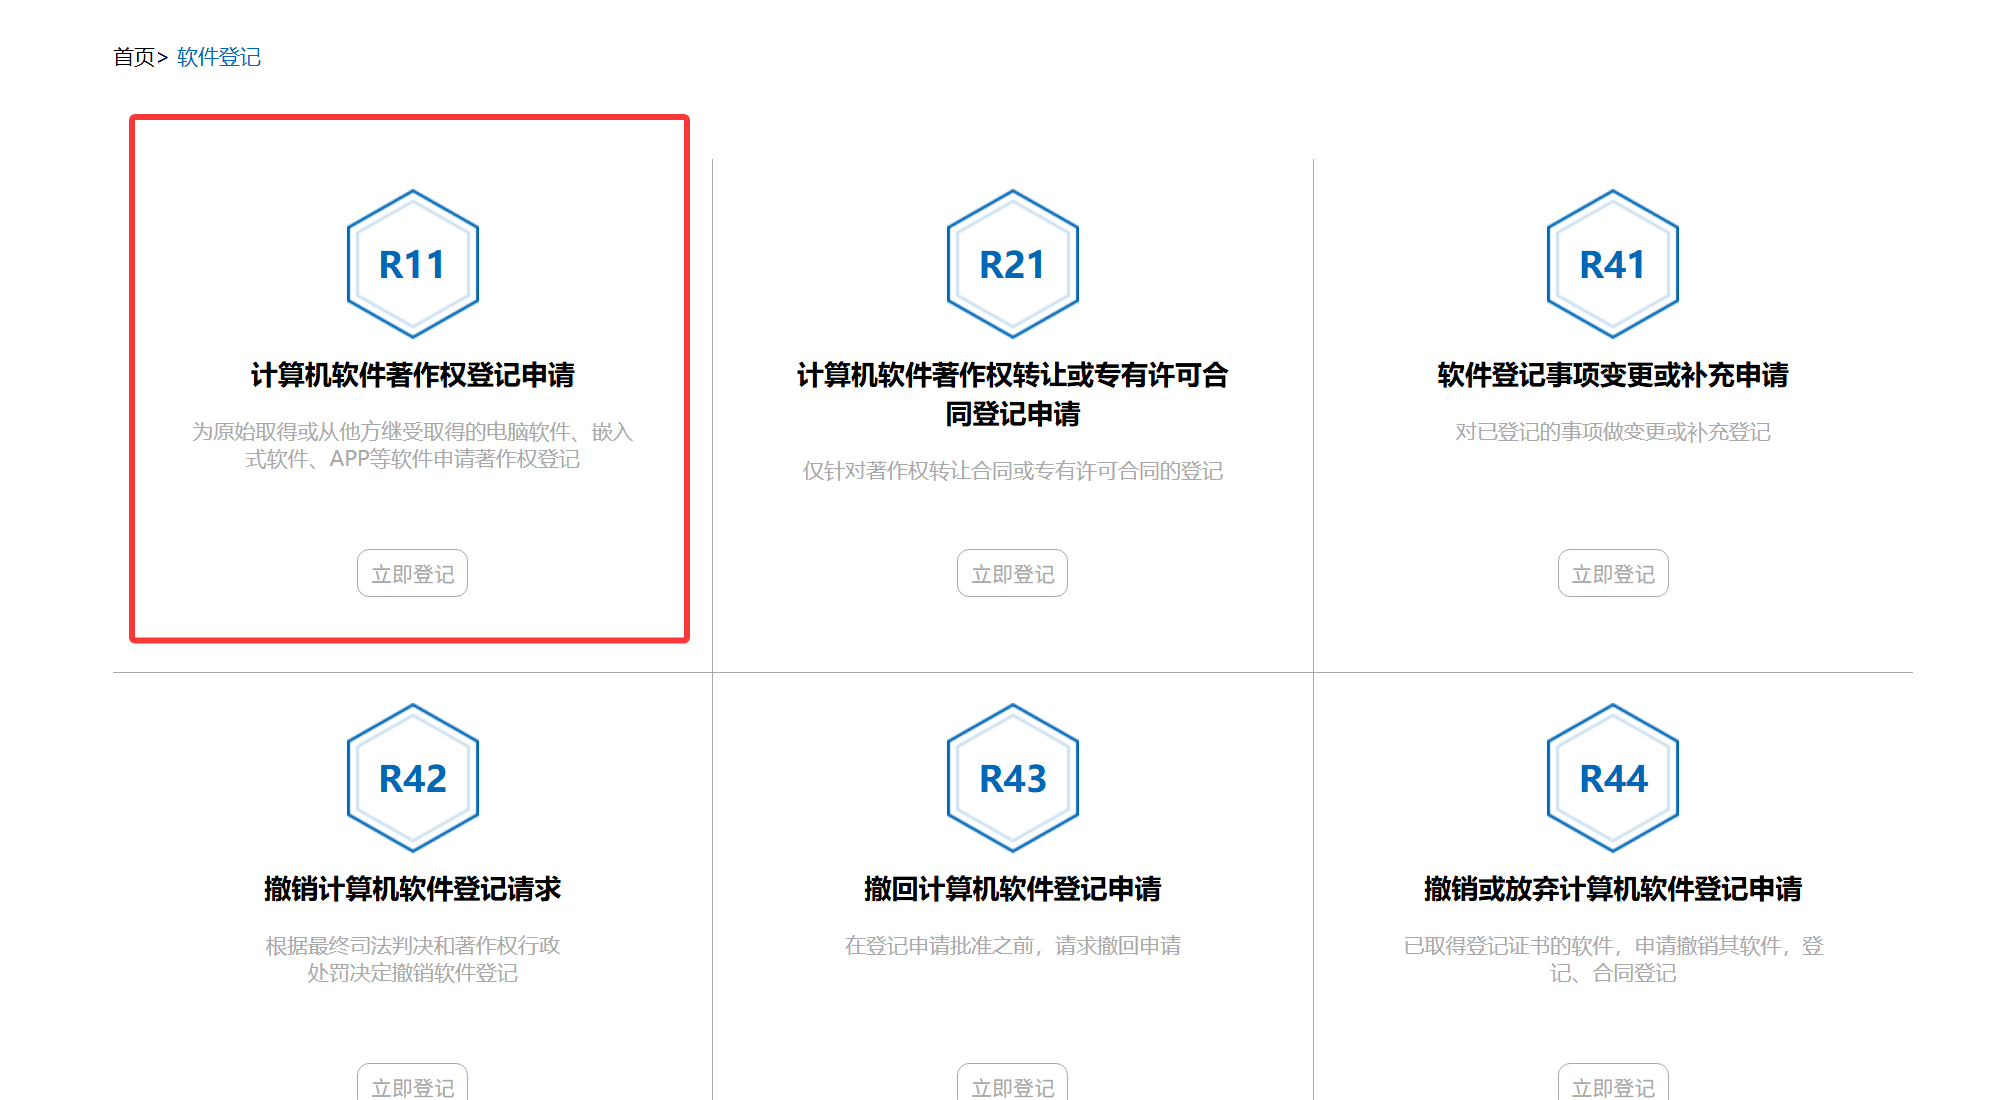
\includegraphics[width=0.99\linewidth]{figures/screenshot001}
	\caption{软件登记页面}
	\label{fig:screenshot001}
\end{figure}

登记类型选择R11，登记证书类型为原始取得。


\newpage
\section{软件简介}

\textbf{下述内容均为材料中必须有的内容，可以在这个基础上增加，但是不能减少必要内容。}

\subsection{编写目的}

\subsection{使用对象}

\subsection{使用范围}


\newpage
\section{产品概述}

\subsection{产品框架}

\subsection{系统架构}

\subsection{模块描述}

\newpage
\section{软件开发说明}

\subsection{软件界面}

\subsection{交互说明}

\subsection{对外接口说明}

\subsection{数据说明}

\subsection{函数实现说明}

\subsection{用户操作接口说明}

\newpage
\section{软件测试说明}

\subsection{手动测试说明}

\subsection{边界测试说明}

\newpage
\section{软件总结与未来设计目标}

\subsection{软件总结}





\subsection{未来设计目标}






 %包括主体的全部内容

\end{document}